%!TEX root = ../report.tex
\chapter{Experiments}
\label{experiments}
In this chapter the experimental results are outlined. The experimental method is outlined in chapter~\ref{method}. For the experiment, a number of simulation runs are recorded in USAR Sim. The map is then 

\section{Experimental Runs}
\subsection{Map 1: IranOpen 2012 - Pre 2}
This map was used in the Iran Open 2012 competition for the second preliminary round \cite{iran2012}. The map features a grey hospital-like environment with grey tiled floors and walls. In figure~\ref{fig:screenshot-map1} a screenshot of the environment is shown.

\begin{figure}[ht]
\centering
\subfigure[Map 1]{
	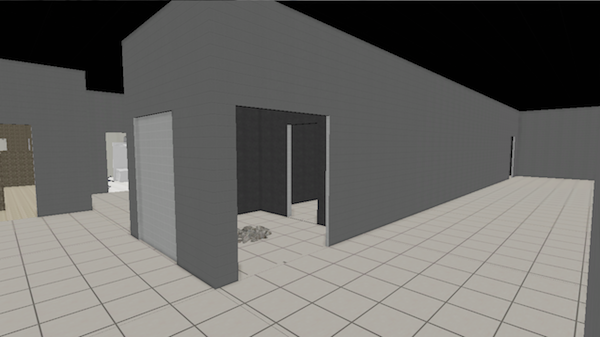
\includegraphics[width=0.4\textwidth]{images/experiment/screenshot-iro2012-pre2.png}
	\label{fig:screenshot-map1}
}
\caption{Screenshots of the maps in the simulation.}
\label{fig:screenshots}
\end{figure}

\subsection{Map 2}
Gotta make a second run.

\subsection{Map 3}
Gotta make a third run.

\section{Confidence measures}


\section{Map segments}

\section{Stitching}

\section{Results}